\section{Méthode de Newton-Raphson}
Dans cette partie, la méthode de Newton-Raphson a été implémentée pour résoudre un système d'équations non linéaires. Cette méthode permet de donner une approximation de la racine de l'équation, qu'il s'agisse d'une équation unidimensionnelle ou multidimensionnelle.

\subsection{Newton-Raphson standard}
Soit $f : \mathbb{R}^n \to \mathbb{R}^n$ définie comme suit :


fonction ici


La jacobienne de cette fonction est la matrice des dérivées partielles selon chaque variable de cette fonction.


jacobienne ici


Le principe de la méthode peut être résumé comme suit :
\begin{itemize}
\item Étant donné un vecteur initial $U_0$, il faut trouver un vecteur $U$ tel que pour tout $\epsilon$ petit $ |f(U)| \le \epsilon $.
\end{itemize}

Pour trouver ce vecteur, l'algorithme doit trouver un vecteur $V$ qu'il faut ajouter au vecteur $U$
pour approcher $f(U+V)$ de $0$.
Il est possible de remplacer $f(U+V)$ par $f(U) + J(U) \cdot V$, ainsi il faut résoudre l'équation $J(U) \cdot H = -f(U)$.
Ceci va être fait en utilisant la fonction \emph{numpy.linalg.lstsq}.

Ce processus sera répété au plus $N_{max}$ fois.
On peut donc conclure que cet algorithme est de complexité $O(N_{max} \times c)$ avec c la complexité de \emph{numpy.linalg.lstsq}.

\subsection{Newton-Raphson avec du backtracking}
La méthode de Newton-Raphson permet bien de trouver la racine, mais pas dans tous les cas, voir figure~\ref{fig:p1-cvg},
c'est pour cela qu'on va utiliser une méthode nommée du backtracking qui permet d'améliorer la
convergence vers cette racine.
Pour ceci, on ajoute des lignes de code qui permettent de vérifier si la condition
$|f(U + \alpha \times V)|\le|f(U)|$ est vérifiée ou pas. On a essayé de diviser $\alpha$ par deux à chaque
itération mais on a rapidement remarqué que la convergence n'est pas assurée. On a donc dû diviser
$\alpha$ par $1.1$.


Pour conclure, on remarque bien que Newton-Raphson avec du backtracking converge vers la racine
contrairement à celle standard selon la figure~\ref{fig:p1-cvg}.
\begin{figure}[htbp]
\centering
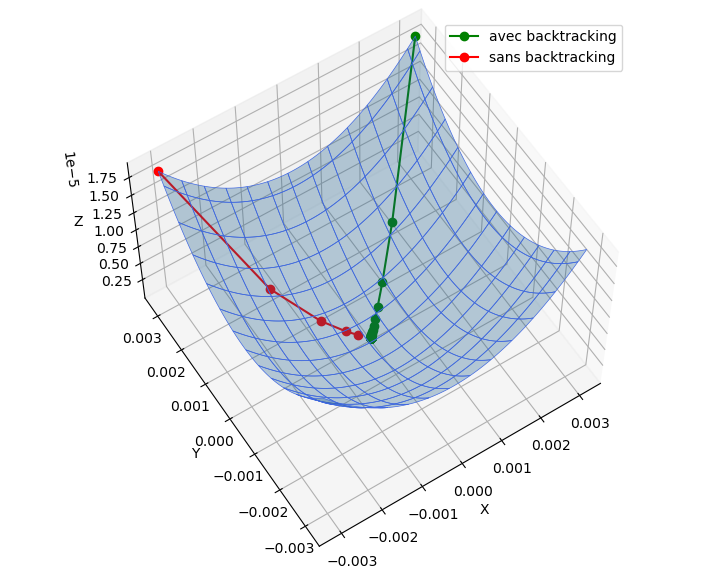
\includegraphics[width=0.65\textwidth]{res/fast_convergence_bt.png}
\caption{Newton-Raphson avec et sans backtracking}
\label{fig:p1-cvg}
\end{figure}
Mais ceci nous coûte en complexité puisque la complexité de Newton-Raphson avec du backtracking
est égale à $O(a \times N_{max} \times c)$ avec c la complexité de \emph{numpy.linalg.lstsq}.